%\subsection{Experiment}
%\label{sec:experiment}

\newcommand{\takeaway}[1]{
\vspace{6pt}
\noindent\fbox{\parbox{\textwidth}{#1}}
\vspace{6pt}
}

 We would like to evaluate the efficiency
 of our algorithms and compare it with \ucalg ~and \ucbfalg ~algorithms.
 Efficiency is computed in terms of wall-clock time.
 In this study, we designed an experiment from
 the same benchmark suite used for evaluation of the \ucalg ~and \ucbfalg ~algorithms in \cite{Ghass16}.
 The benchmark contains 476 Lustre models
 published in~\cite{Hagen08:FMCAD} augmented
with 81 additional models from industrial case studies ~\cite{QFCS15:backes,hilt2013}.
 Most of
the benchmark models from~\cite{Hagen08:FMCAD} are small (10kB or less,
with 6-40 equations) and include a range of hardware benchmarks and
software problems involving counters.
The industrial cases are much
larger: around 80kB with over 600 equations.
Each benchmark model has a single property to analyze.
For each test model, we computed \aivcalg , \ucalg , and \ucbfalg ~algorithms
in a configuration with
the \texttt{Z3} solver and the fastest mode of \texttt{JKind} (running k-induction and PDR in parallel). The experiments
were run on an  Intel(R) i5-4690, 3.50GHz,
16 GB memory machine.\footnote{\noindent ~The benchmarks, all raw experimental results,
  and computed data are available on \cite{expr}.}

\begin{figure}[t]
 \centering
  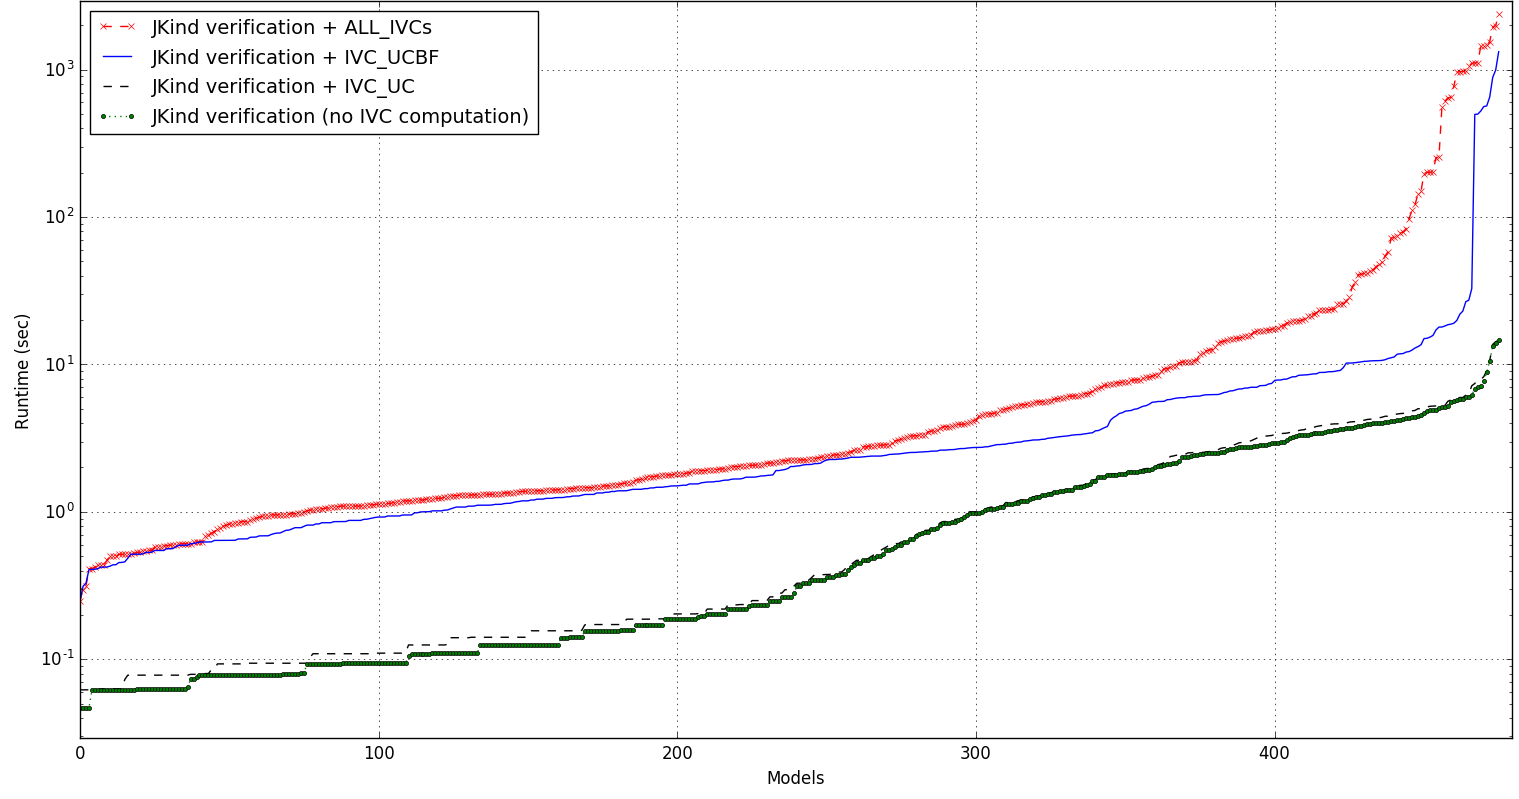
\includegraphics[width=\textwidth]{figs/performance-sorted.png}
  \label{fig:performance}
  \vspace{-0.2in}
  \caption{Runtime of \aivcalg, \ucbfalg, and \ucalg ~algorithms}
\end{figure}

One technical issue that needs to
be handled in any implementation of the \aivcalg ~algorithm,
is about the undecidability of the model checking algorithms;
in each iteration of the \texttt{while} loop, Algorithm~\ref{alg:aivc}
has to decide on the adequacy of a given set $M \subseteq T$ (line 8).
This decision should be made by the use of a proof method that
tries to prove the property $P$ over $M$. Although we know that $(I, T) \vdash P$,
there is no guarantee that we can determine whether or not any $M \subset T$ is adequate.
Therefore, in practice, we have to set some boundaries
(over depth/time of the model checking algorithm) in each iteration.
In our implementation, we set a timeout based on the time a property takes to be proved.
Since before starting the \aivcalg ~algorithm, the property has to be proved,
we obtain its required \emph{proof-time}.
Then, the timeout we set for each iteration is ($60 sec  + 10 \times$ \emph{proof-time}).
When the \texttt{while} loop times out for $M$ in line 8 of Algorithm~\ref{alg:aivc},
we treat $M$ as an \emph{inadequate} set because
when the adequacy of $M$ is undecidable,
 the adequacy of all its subsets are undecidable too. So, if we consider it as inadequate, line 13 will prune off $M$ and all its subsets from the search space. \ela{~~Ela: do you have better justification? }
Even so, in our benchmarks, there have been a few models containing iterations with timeout.

We measured the performance overhead of the algorithms over the time
necessary to find a proof using inductive model checking. Fig. \ref{fig:performance}
 allows a visualization of the  overhead  of the \aivcalg ~algorithm  in  comparison  with \ucalg ~and \ucbfalg, which is also summarized in Table \ref{tab:overhead}.
 The running time of the algorithms is also summarized in Table \ref{tab:runtime}.
 Note that the \aivcalg ~algorithm could have had better (worse) performance
 if timeout had been set lower (higher).

\begin{table}
  \caption{Overhead of different algorithms}
   \vspace{-0.1in}
  \centering
  \begin{tabular}{ |c||c|c|c|c| }
    \hline
     algorithm & min & max & mean & stdev \\[0.5ex]

    \hline
    \aivcalg   & 13.642\% & 101034.615\% & 2544.399\% & 7764.159\% \\[0.5ex]
    \ucbfalg &   14.092\% & 111124.432\% &  882.018\% & 1512.071\%\\[0.5ex]
    \ucalg&  0.00\%  & 100.00\%   & 10.226\% & 11.718\% \\[0.5ex]
    \hline
  \end{tabular}
  \label{tab:overhead}
\end{table}

\begin{table}
  \caption{Runtime of different computations}
   \vspace{-0.1in}
  \centering
  \begin{tabular}{ |c||c|c|c|c| }
    \hline
      runtime (sec)& min & max & mean & stdev \\[0.5ex]
    \hline\hline
    \emph{\small{proof-time}}    & 0.047 & 14.617 & 1.299 & 1.940 \\[0.5ex]
    \aivcalg    & 10.125 & 2375.058& 58.884 & 256.529 \\[0.5ex]
    \ucbfalg &   0.248 & 1323.515 &  17.247& 104.838\\[0.5ex]
    \ucalg&  0.0  & 1.422  & 0.084 & 0.184 \\[0.5ex]
    \hline
  \end{tabular}
  \label{tab:runtime}
\end{table}

\takeaway{Computing all minimal Inductive Validity Cores with the \aivcalg ~algorithm is as nearly expensive as computing one single minimal Inductive Validity Core with the \ucbfalg  ~algorithm.
\ela{Ela: is that fair to say??}} 